\section{Library Language}
The Domain Specific Language (DSL) we have created is an attempt at modelling a Library system. We have a chosen the context of a public library as opposed to a specialised facility such as a university or law library. The DSL is naturally constrained by our development tool and as such  is comprised of three main entities: Objects, Relationships and Roles. These entities are described in the following sections. 

\subsection{Objects}
Objects represent physical entities such as loanable items, library equipment and people such as library users and employees. Examples of Objects within the system include a book shown in Figure~\ref{fig:objbook}.

\begin{figure}[H]
  \centering
  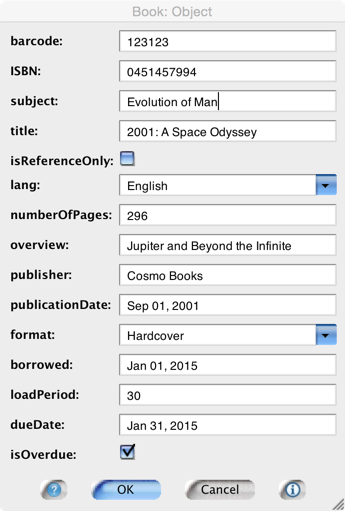
\includegraphics[width=0.5\textwidth]{obj_book}  
  \caption{A book object from the DSL.}
  \label{fig:objbook}
\end{figure}

% \begin{figure}[H]
%   \centering
%   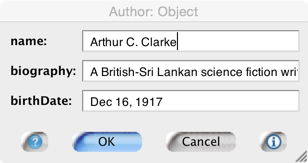
\includegraphics[width=1\textwidth]{obj_author}
%   \caption{A book object from the DSL.}
%   \label{fig:objauth}
% \end{figure}

% \begin{figure}[H]
%   \centering
%   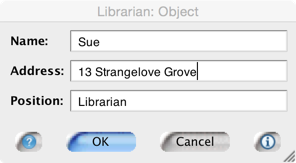
\includegraphics[width=1\textwidth]{obj_librarian}
%   \caption{A book object from the DSL.}
%   \label{fig:objlibr}
% \end{figure}

% \begin{figure}
%   \centering
%   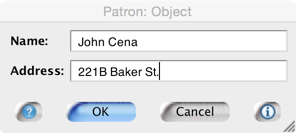
\includegraphics[width=1\textwidth]{obj_patron}
%   \caption{A book object from the DSL.}
%   \label{fig:objpat}
% \end{figure}







\subsection{Relationships}
Relationships describe methods by which objects within the DSL may interact. For example, as shown in Figure~\ref{fig:authrel}, within our system an Author may have a \emph{wrote} relationship with a Book object.

\begin{figure}[H]
  \centering
  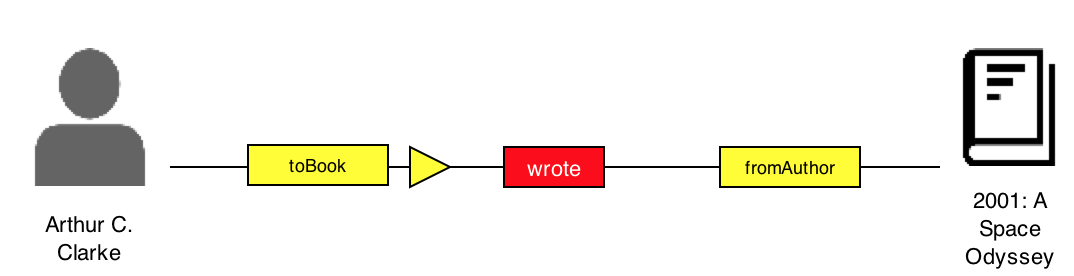
\includegraphics[width=.8\textwidth]{rel_wrote}
  \caption{A \emph{wrote} relationship from Author to Book}
  \label{fig:authrel}
\end{figure}
% 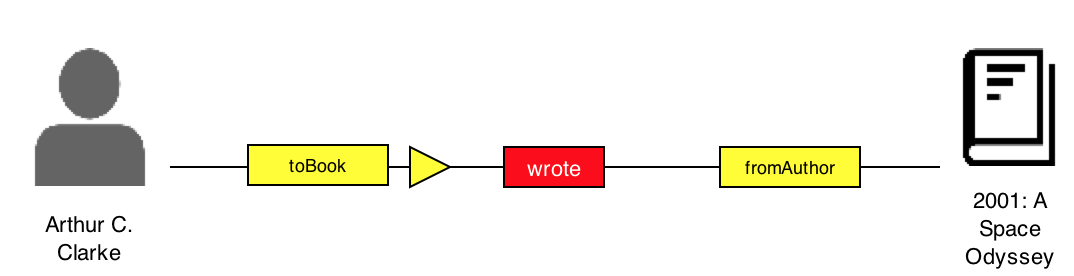
\includegraphics[width=1\textwidth]{rel_wrote}
% 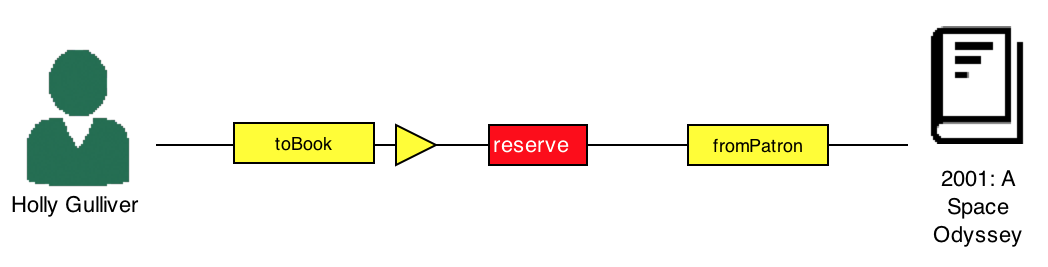
\includegraphics[width=1\textwidth]{rel_reserve}
% 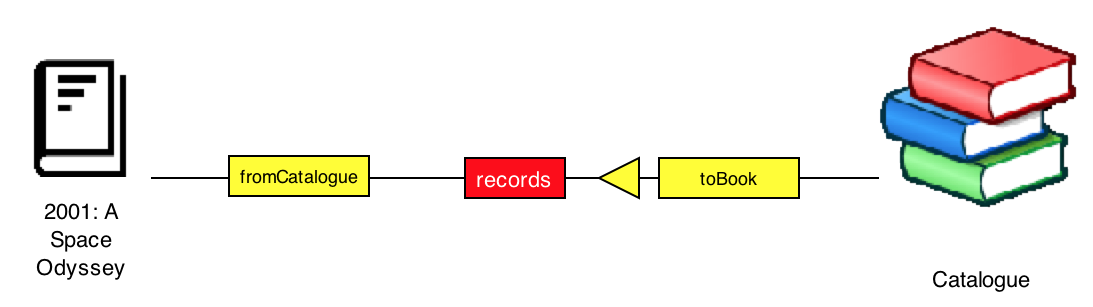
\includegraphics[width=1\textwidth]{rel_records}


\subsection{Roles}
Roles define restrictions on the types of objects that may exist on either end of a relationship between those objects. For example, as shown in Figure~\ref{fig:resrole}, a Patron make take one end of the \emph{reserves} Role to Book.

\begin{figure}[H]
  \centering
  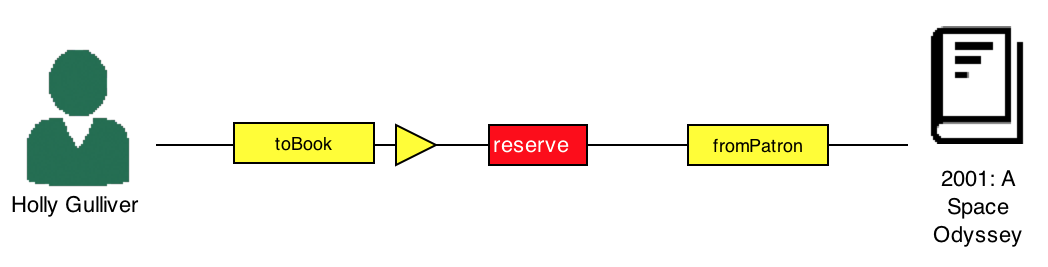
\includegraphics[width=.8\textwidth]{rel_reserve}
  \caption{A Patron has a role in the Relationship \emph{reserves} to Book}
  \label{fig:resrole}
\end{figure}

\subsection{Constraints}
In addition to the Relationship and Role entities constraints may be defined surrounding the semantics of relationships. These constraints fall into four categories:\newline
\textbf{Connectivity}: cardinality and type of some shit about the thing with a thing. \newline
\textbf{Occurrence}: constraint surrounding the number of a unique objects may appear in a graph.\newline
\textbf{Uniqueness}: uniqueness constraints for property values such as ID.\newline
Creating and applying constraints allows further development and enrichment of DSL semantics.


